\documentclass{article}
\usepackage[affil-it]{authblk}
\usepackage{graphicx}
\usepackage[space]{grffile}
\usepackage{latexsym}
\usepackage{textcomp}
\usepackage{longtable}
\usepackage{multirow,booktabs}
\usepackage{amsfonts,amsmath,amssymb}
\usepackage{natbib}
\usepackage{url}
\usepackage{hyperref}
\hypersetup{colorlinks=false,pdfborder={0 0 0}}
%\usepackage{latexml}
\usepackage[utf8x]{inputenc}
\usepackage[english]{babel}




\begin{document}

\title{Cognitive Limitations of Human Bayesian Learning}


\author{Thomas}
\affil{Affiliation not available}

  
\author{Johannes Castner}
\affil{Affiliation not available}
  
\author{Nate Neligh}
\affil{Affiliation not available}
  



\date{\today}

\bibliographystyle{plain}

\maketitle 




\begin{figure}[h!]
\begin{center}
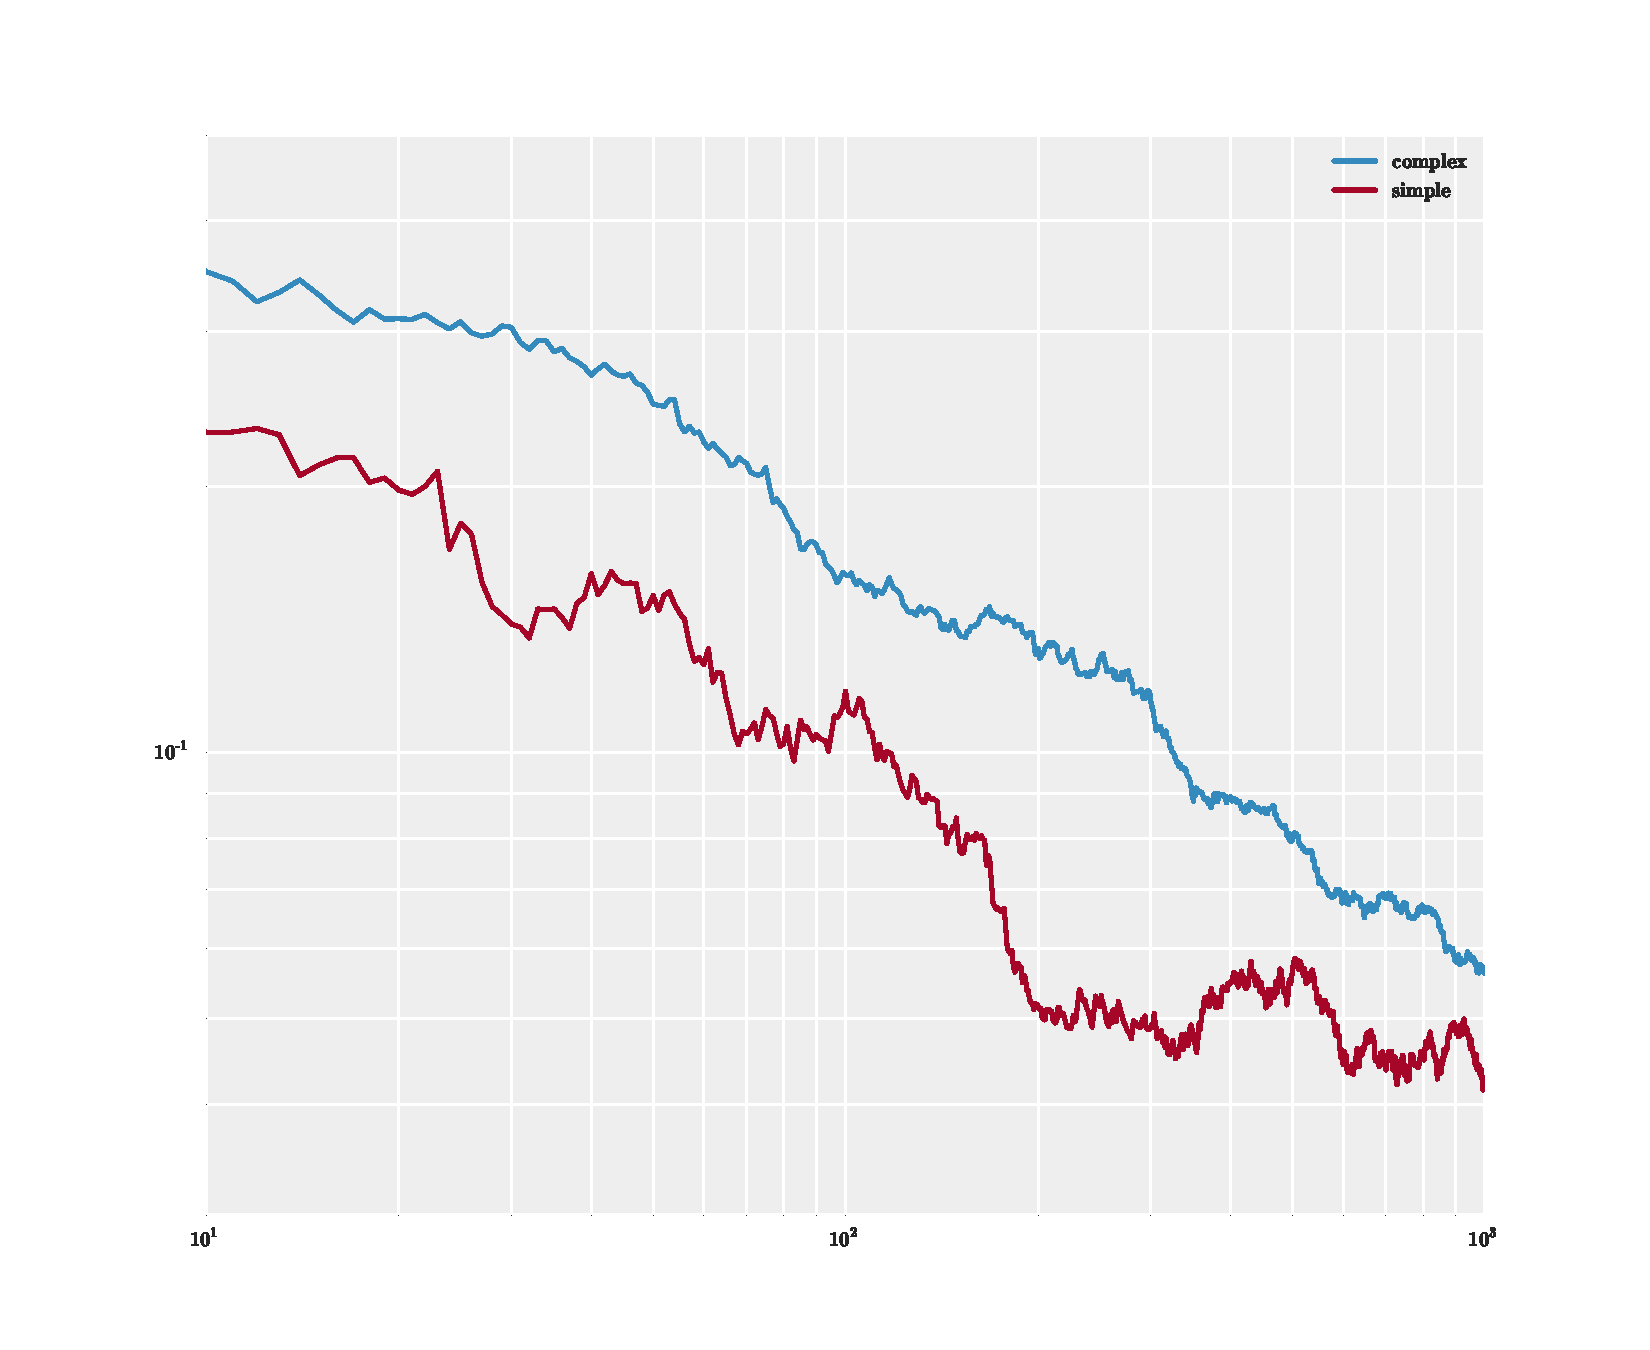
\includegraphics[width=0.7\columnwidth]{figures/empiricalConvergenceLogLog/empiricalConvergenceLogLog}
\caption{\label{fig:fully_rational}
Replace this text with your caption%
}
\end{center}
\end{figure}

To do list:
\begin{itemize}
\item (Johannes) Explanation rational Bayesian convergence being equal $\sqrt{t} = t^{1/2}$
\\
This follows from the Central Limit Theorem and from the fact that a rationally updated dirichlet conjugate prior acts as a counts model. For details see the following Wikipedia articles: \href{https://en.wikipedia.org/wiki/Central_limit_theorem}{Central Limit Theorem} and \href{https://en.wikipedia.org/wiki/Dirichlet_distribution}{Dirichlet Distribution}. 
\item (Thomas) Explain the Hawkes Poisson Process as a {\bf candidate} model in this context of bounded rationality
\item (Thomas) Check dynamics as a function of 2 minutes sessions $\rightarrow$ Is there any coherent pattern between spikes and 2 minutes periods
\item (Johannes) Compute  matrices of distances between models as a function of time: The output should be triangular matrices 
\item (Johannes) Learning models in Economics
\end{itemize}
  
  
  
  
  

\begin{figure}[h!]
\begin{center}
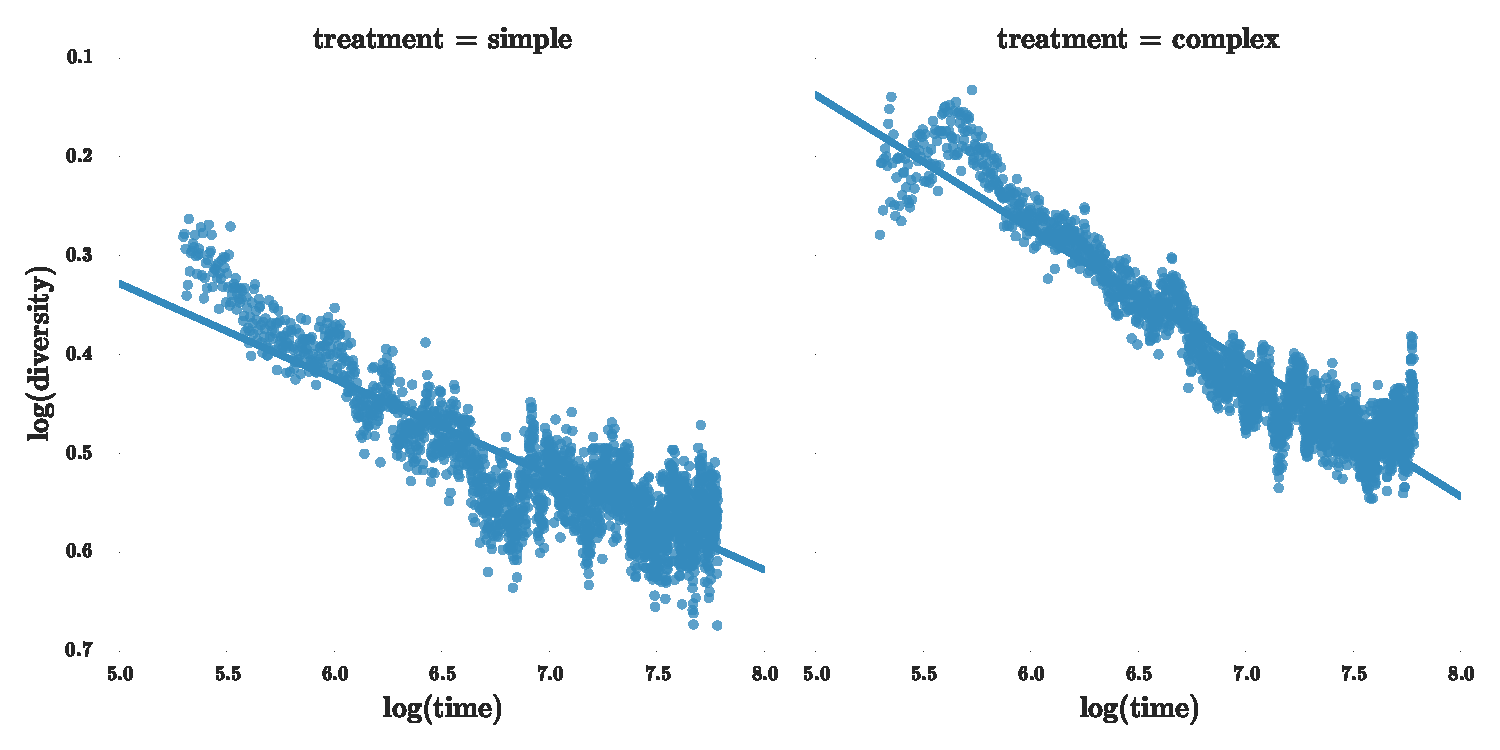
\includegraphics[width=1\columnwidth]{figures/DiversityLogLog/DiversityLogLog}
\caption{%
}
\end{center}
\end{figure}

$\frac{Diversity}{\text{Distance from true process}}=C*t^{\alpha - \beta}$, where $\alpha$ is the rate of decrease in diversity and $\beta$ is the rate of human or collective learning. 
  
  

\begin{figure}[h!]
\begin{center}
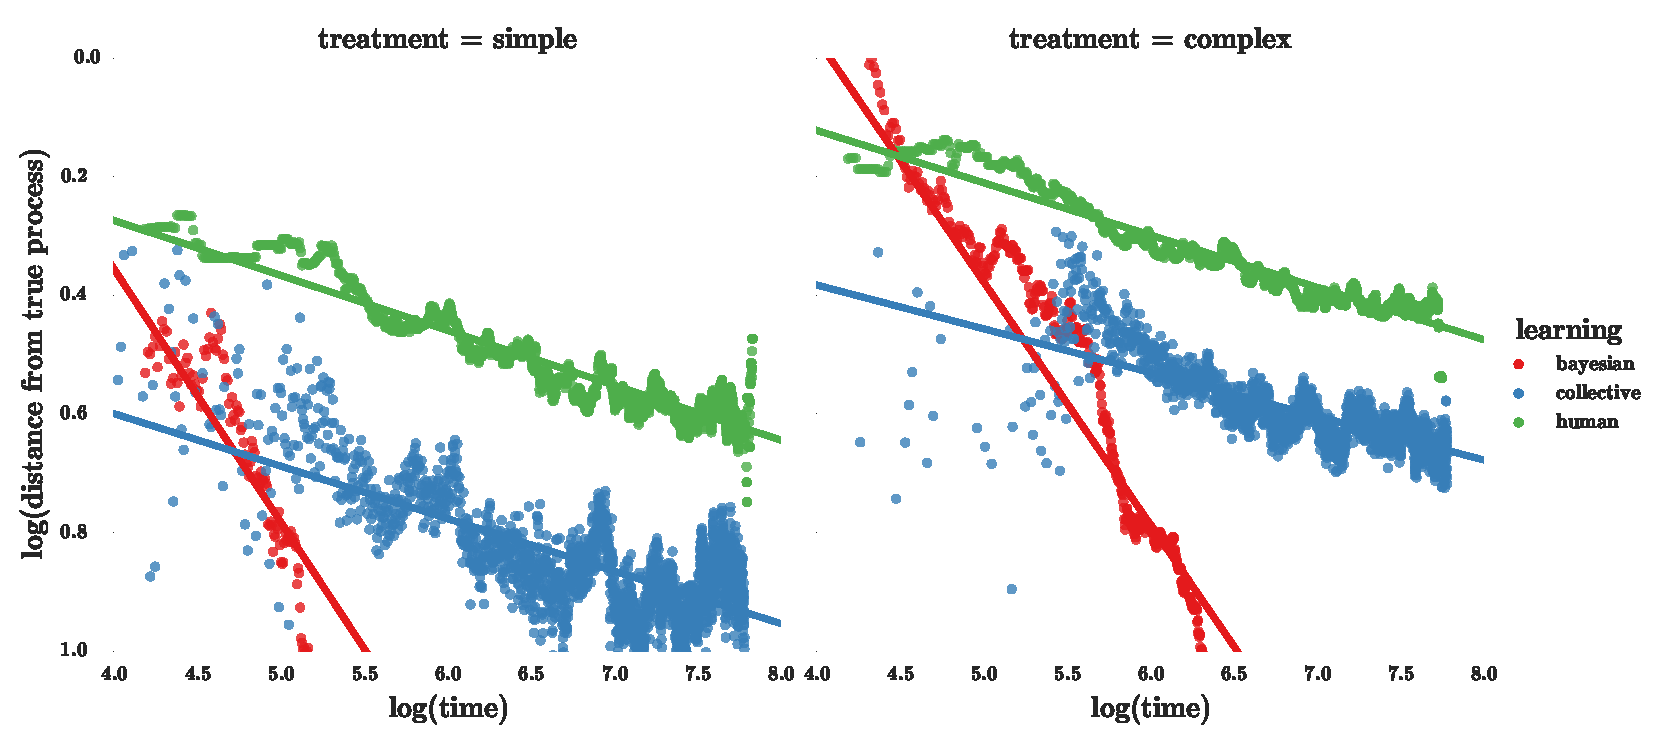
\includegraphics[width=1\columnwidth]{figures/LogLog/LogLog}
\caption{\label{fig:convergence_humans}
caption see text above%
}
\end{center}
\end{figure}

\section{Distribution of step-by-step performance}

Binned (100 bins) density function of distance between 2 steps. This distance can be positive, which is equivalent to adding distance compared to the true model (in red). On the contrary, a negative distance shows improvement (in green). Both sides are heavy-tailed distributions, with very good fits with a power law model (see both insets). However, the exponents are different for improvement (exponent = 2.25), compared to counter performance (exponent, 1.34). This discrepancy explains why on average participants make improvements at a pace of $\alpha = 0.9 = 2.25 - 1.34$ {\bf [formal demonstration needed here $\rightarrow$ it implies a stochastic process with stochastic increment given this distribution, which is equivalent (in my mind) to considering a balanced stochastic component with exponent 1.34 on both sides, and a deterministic drift of 0.09]}. 

The values of the exponents tell us that progress (exponent = 2.25) has its first moment (mean) well defined, but variance diverges. On the contrary, counter performance (exponent = 1.34) has its mean and variance diverge as $n \rightarrow \infty$ (up to some boundaries, which we can see on both side in both insets $\rightarrow$ actually we could fit a power-law with a exponential crossover in the tail, or even better, impose a hard limit which must be 1 on both sides (in theory), i.e. at best (resp. worst) the participant can jump from guessing the worst possible model to the true model (from 1 to 0 $\rightarrow$ -1), (resp. having reached the best model, jump back to the worst (from 0 to 1 $\rightarrow$ 1). The point of maximum density is very close to but smaller than 0 with value -0.01. This 1\% improvement occurs 96\% of participant attempts. {\bf [One may also want to consider the adjustment constants to quantify exactly how much it likely to make a jump of $|\epsilon|$ (either better performance or worse performance)]}.

\begin{figure}[h!]
\begin{center}
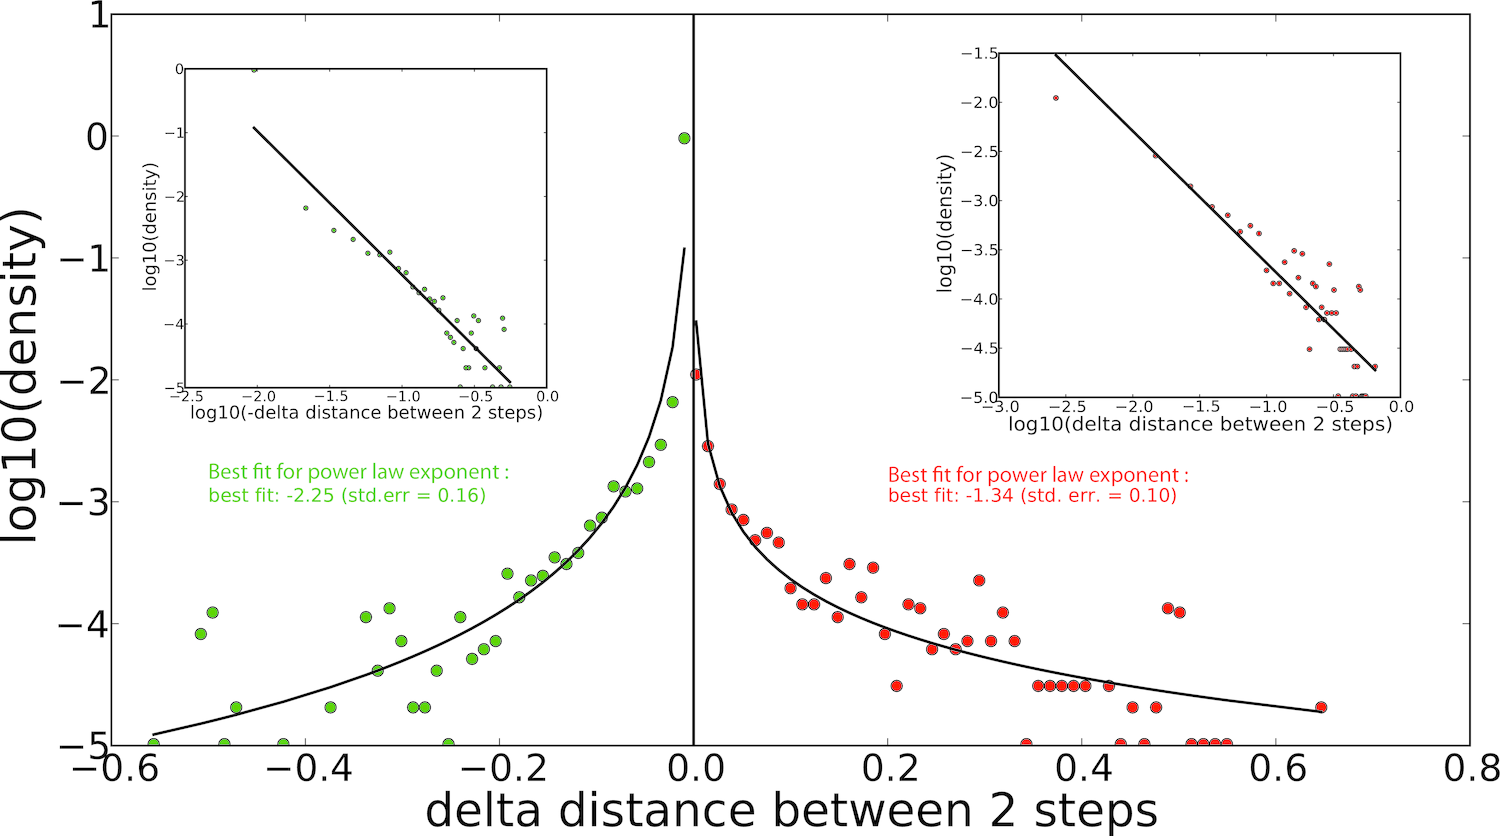
\includegraphics[width=0.7\columnwidth]{figures/pdfPerformance/pdfPerformance}
\caption{Binned (100 bins) density function of distance between 2 steps. This distance can be positive, which is equivalent to adding distance compared to the true model (in red). On the contrary, a negative distance shows improvement (in green). Both sides are heavy-tailed distributions, with very good fits with a power law model (see both insets). However, the exponents are different for improvement (exponent = 2.25), compared to counter performance (exponent, 1.34). This discrepancy explains why on average participants make improvements at a pace of $\alpha = 0.09 = 2.25 - 1.34$ {\bf [mistake here 0.09 $\rightarrow$ 0.9 ! formal demonstration needed here $\rightarrow$ it implies a stochastic process with stochastic increment given this distribution, which is equivalent (in my mind) to considering a balanced stochastic component with exponent 1.34 on both sides, and a deterministic drift of 0.09]}. The values of the exponents tell us that progress (exponent = 2.25) has its first moment (mean) well defined, but variance diverges. On the contrary, counter performance (exponent = 1.34) has its mean and variance diverge as $n \rightarrow \infty$ (up to some boundaries, which we can see on both side in both insets $\rightarrow$ actually we could fit a power-law with a exponential crossover in the tail, or even better, impose a hard limit which must be 1 on both sides (in theory), i.e. at best (resp. worst) the participant can jump from guessing the worst possible model to the true model (from 1 to 0 $\rightarrow$ -1), (resp. having reached the best model, jump back to the worst (from 0 to 1 $\rightarrow$ 1). The point of maximum density is very close to but smaller than 0 with value -0.01. This 1\% improvement occurs 96\% of participant attempts. {\bf [One may also want to consider the adjustment constants to quantify exactly how much it likely to make a jump of $|\epsilon|$ (either better performance or worse performace)]}.%
}
\end{center}
\end{figure}

\section{A metric to measure Exploration and Expoitation}

Intuitively, as people build models and adjust them, they can explore new terrain in model space or they can combine models that they have previously built. How they explore new regions or exploit regions that they have explored before can only be understood if we can measure the degree of current period exploitation and exploration.  Clearly, when people first start building probabilistic models their only choice is to explore new grounds and thus the exploration metric should be maximal at period 0.  This maximum of the exploration metric is arbitrarily set to 1 and its opposite (exploitation) is set to 0.  In fact, at every time period the exploration and exploitation metrics obey the following deterministic relationship: 

exploration$_t$ = 1-exploitation$_t$, 

with exploration$_t$, exploitation$_t$ $\in [0, 1]$. 

The exploration metric is obtained by calculating a particular distance measure, the square-root of the Jensen Shannon Divergence, between a weighted sum of all previous models and the new model. This has the property that models outside of the convex hull of all previous models are maximally explorative and models in the center of the convex hull of all previous models are maximally exploitative, as would seem intuitive.  The convex hull defined by a set of points in a two dimensional space could be thought of as that part of $\mathbb{R}^2$ that lies in the interior when a rubber band is stretched around all of the points. 

\section{Relation between Perfect and Human Bayesian Learning}
It's quite simple but says the difference between perfect Bayesian learning ($BL$) and human learning ($HL$):

\begin{equation}
BL(t) \sim 1/t^{\alpha}~,~with~\alpha = 0.5\\
HL(t) \sim 1/t^{\beta}~,~with~\beta \approx 0.1\\
\label{BHL}
\end{equation}
 
Hence, 
\begin{equation}
HL(t) \sim BL(t)^{\gamma}~,~with~\gamma \approx 1/5.
\end{equation}

One shall also consider the initial conditions: what are the performances at $t=0$ for $BL$ and $HL$ in both simple and complex cases $\rightarrow$ this super important because it's the only visible difference between the 2 games (simple and complex)!

So the $\gamma \approx 1/5$ is a measure of the discrepancy between a perfect learner and a human learner (on average). As the volatility is high, we shall however expect better or worse human learners compared to this average, but in general, time performance may converge in the following way,

\begin{equation}
Time~Performance = \frac{\Delta Distance(t)}{\Delta t} \rightarrow 0~as~t\rightarrow \infty,
\end{equation}

which is consistent with empirical results given by \ref{BHL}.


  
  
  
  
  

\section{Propositions for explaining the difference between BL and HL}

This shall be supported by empirical evidence, but there are not zillions of possibilities: It certainly takes more time to come up with models which significantly reduce the distance to the true model. Reasons may be 

\begin{itemize}
\item lack of creativity
\item lack of trying (procrastination)
\item memory afterglow of already tested solutions (i.e., returning to already tested models which do not bring much)
\item increased time to think of new solutions leading to substantial improvement (looks like procrastination in some way), or to perform integration of various solutions tested previously.
\end{itemize}

I think we can formulate tests for nearly all these possibilities.

  

\subsection*{Rationale for a Hawkes Conditional Poisson Procees}
Bayesian learning is based on the accumulation of experience through multiple trials. Figure \ref{fig:fully_rational} shows a fully rational Bayesian learning starting with a uniform prior that an equal probability to every outcome. Starting from this uniform guess, a fully rational player builds a catalog of configuration and how they perform (i.e., the perceived probability that they are the true model). As learning occurs, new configurations are proposed, which rely on past configurations, presumably the most performing ones. The fully rational player has access to all configurations and their performance with the same perfect memory. 

On the contrary, players with bounded rationality, e.g., human beings with limited memory and cognitive capabilities, can only withdraw a subset of the full catalog of configurations already tested. For instance, it is easier to recall a configuration which has been tested in the recent past, rather than long time ago.

In both cases (fully rational and bounded rational), the probability that the new configuration will inherit from recently tested configurations is higher, compared to old configurations. The reason is that latter configurations incorporate information for former configurations (this should be the explanation for the decay $\sim t^{-0.5}$ observed in Figure \ref{fig:fully_rational}). 

We posit that bounded rational players suffer from (i) their inability to perfectly integrate information in the new configurations the design and from (ii) the fact that they may have hard remembering all configurations, in particular those tested further in the past.

The memory issue can be understood as a problem of influence with memory, which is perhaps long-range. In the latter case, the decay of influence of past events shall follow, e.g., a power law, which may at least in part explain the super small exponent $\alpha = 0.09$ observed (see Figure \ref{fig:convergence_humans}).

Influence with memory, resp. long-range memory, may be modeled with conditional Poisson processes. Self-excited Hawkes conditional Poisson processes \cite{Hawkes_1974}, are particularly handy to account for exogenous shocks, perturbing a system, and triggering endogenous reactions by this system \cite{Crane_2008}. The Hawkes conditional Poisson process is defined by the intensity $I(t)$ of events at time $t$, given by
\begin{equation}
I(t)= \lambda(t) + \sum_{i | t_t<t}  f_i \phi(t-t_i)~,
\label{eq:Hawkes}
\end{equation}
where $\{t_i, i=1, 2, ...\}$ are the timestamps of past events, $\lambda(t)$ is the exogenous rate of events, $f_{i}$ is the average fertility of events $i$ that quantifies the number of daughter (first generation) events, and $ \phi(t-t_i)$ is the memory kernel, which reflects the long-memory effects of task prioritization, and economy of time as a non storable resource \cite{Maillart_2011}. Here, the main exogenous shock is $\lambda(t_{0})$, with $t_{0}$ the first day of the Astro Hack Week. The second term of the right hand side of equation (\ref{eq:Hawkes}) represents the endogenous response to exogenous shocks (i.e., here, the response to the initial shock at $t_{0}$). 

{\bf NB: I just copied paste from another paper. It may be that the model should be adapted, or we might have to borrow from other theories. I just provide it here as a starting point for discussion on possible dynamics occurring in relation with cognitive processes involving memory.}
  
  
  
  
  
  

\section{Rational (Bayesian or Frequentist) Learning}

The basic idea is that the incentives in the game are such that for a Bayesian (rational) learner it is optimal to express her model as the maximum point of her posterior distribution after observing counts of joint outcomes of the $k$ binary variables. In other words, all of the information is in the frequency counts of the observed joint states of the system because in the time dimension the observations and payoffs are i.i.d. and all that matters are the signals which are in the form of observations of the states of the other variables (the covariates). 
What this essentially means is that a rational Baysian learner will build a model that in the limit and in practice quite quickly converges to a normalized frequency count of the joint outcomes in the cross domain of the system under observation. Thus, a Bayesian learner learns at the same speed at which the normalized frequency counts of the system converge to their limiting distribution. The Central Limit Theorem determines the rate of convergence of normalized frequency counts to their long-term probabilities to be $\mathcal{O}( t^{-\frac{1}{2}})$, where $t$ is a time index determined by the entry of new information, or some constant times the entry of new information. So that if every 240 seconds a new piece of information is revealed, we can say that $t=240*s$, where $s$ is an index on each data point. The Bayesian learner then converges to the truth as 

$\log((240*s)^{-\frac{1}{2}}) =-\frac{1}{2}(\log(240) + \log(s))$

$= \beta_{rational} * (\log(240)+\log(s))$

$= \alpha_{rational}+\beta_{rational}\log(s).$  

Clearly, $\beta_{rational}=-\frac{1}{2}.$ 

In general, $\alpha_{rational}$ is the logarithm of the period 1 measure:

$\alpha_{rational}=\beta_{rational} * \log(\text{SF}*\gamma_{rational})$,

where SF is the scaling factor measured in some time unit such as seconds (240 in the above case) and $\gamma_{rational}$ is a parameter determined by the prior.  Note that scale free here means that the speed of convergence does not depend on how often data is observed as long as it is observed at some constant interval. 

Since there is no such thing as a "rational" prior, $\alpha_{rational}$ is completely arbitrary but in our framework it is forced to be negative as $e^{\alpha}$ here is the diversity or distance measure at time $1$ and those measures take on values in $[0, 1]$. The only constraint on $\alpha_{rational}$ then is that $e^{\alpha}\in [0, 1]$ and else nothing more can be said about it. A rational learner starts with a disposition that is arbitrarily far from or close to the truth and the log distance from the updated disposition to the limiting distribution converges at a rate $-\frac{1}{2}*\log(t)$.  Putting everything together, we have that 

$E_{rational}(w_{i,t}) =e^{\alpha}*t^{-\frac{1}{2}},$

where $E_{rational}$ is the expectation when the rational case is assumed of some distance measure $w(\cdot) \in [0,1]$ of the $i$s learner at time $t$ to the true limiting distribution, remembering that $t$ is a positive multiple (a time interval) of an index, $s$ on an indexed i.i.d data series. 

\section{What we can observe from Matrices} We have produced two types of matrices, which allow to get a visual glimpse of the search process by participants. A representative example of these matrices is shown below in Figure ???. Patterns are diverse and described in more detail on the Figure and on its caption. But the triangle matric {\bf A} shows well the search process performed by the participant: High contrasted boundaries show disruptive model propositions, well homogeneous color rectangle show stability of contiguous models, perhaps with some slight iterative improvement (it's hard to see from the figure actually). Yellowish Horizontal stripes show integration of many former models, while blueish horizontal stripes, show exploration of solutions remote from all solutions proposed beforehand.  

It's unclear how we can exploit this visual insights so far, but it reminds me of some organization science theories, involving research and development versus production, where a balance is desirable, between searching for radical solutions and exploiting them for converging e.g., towards a product \cite{March_1991}. This theory certainly applies to individuals, yet the same phenomenon shall have already been documented in cognitive science {\bf [references are needed]}. 
  
  

\begin{figure}[h!]
\begin{center}
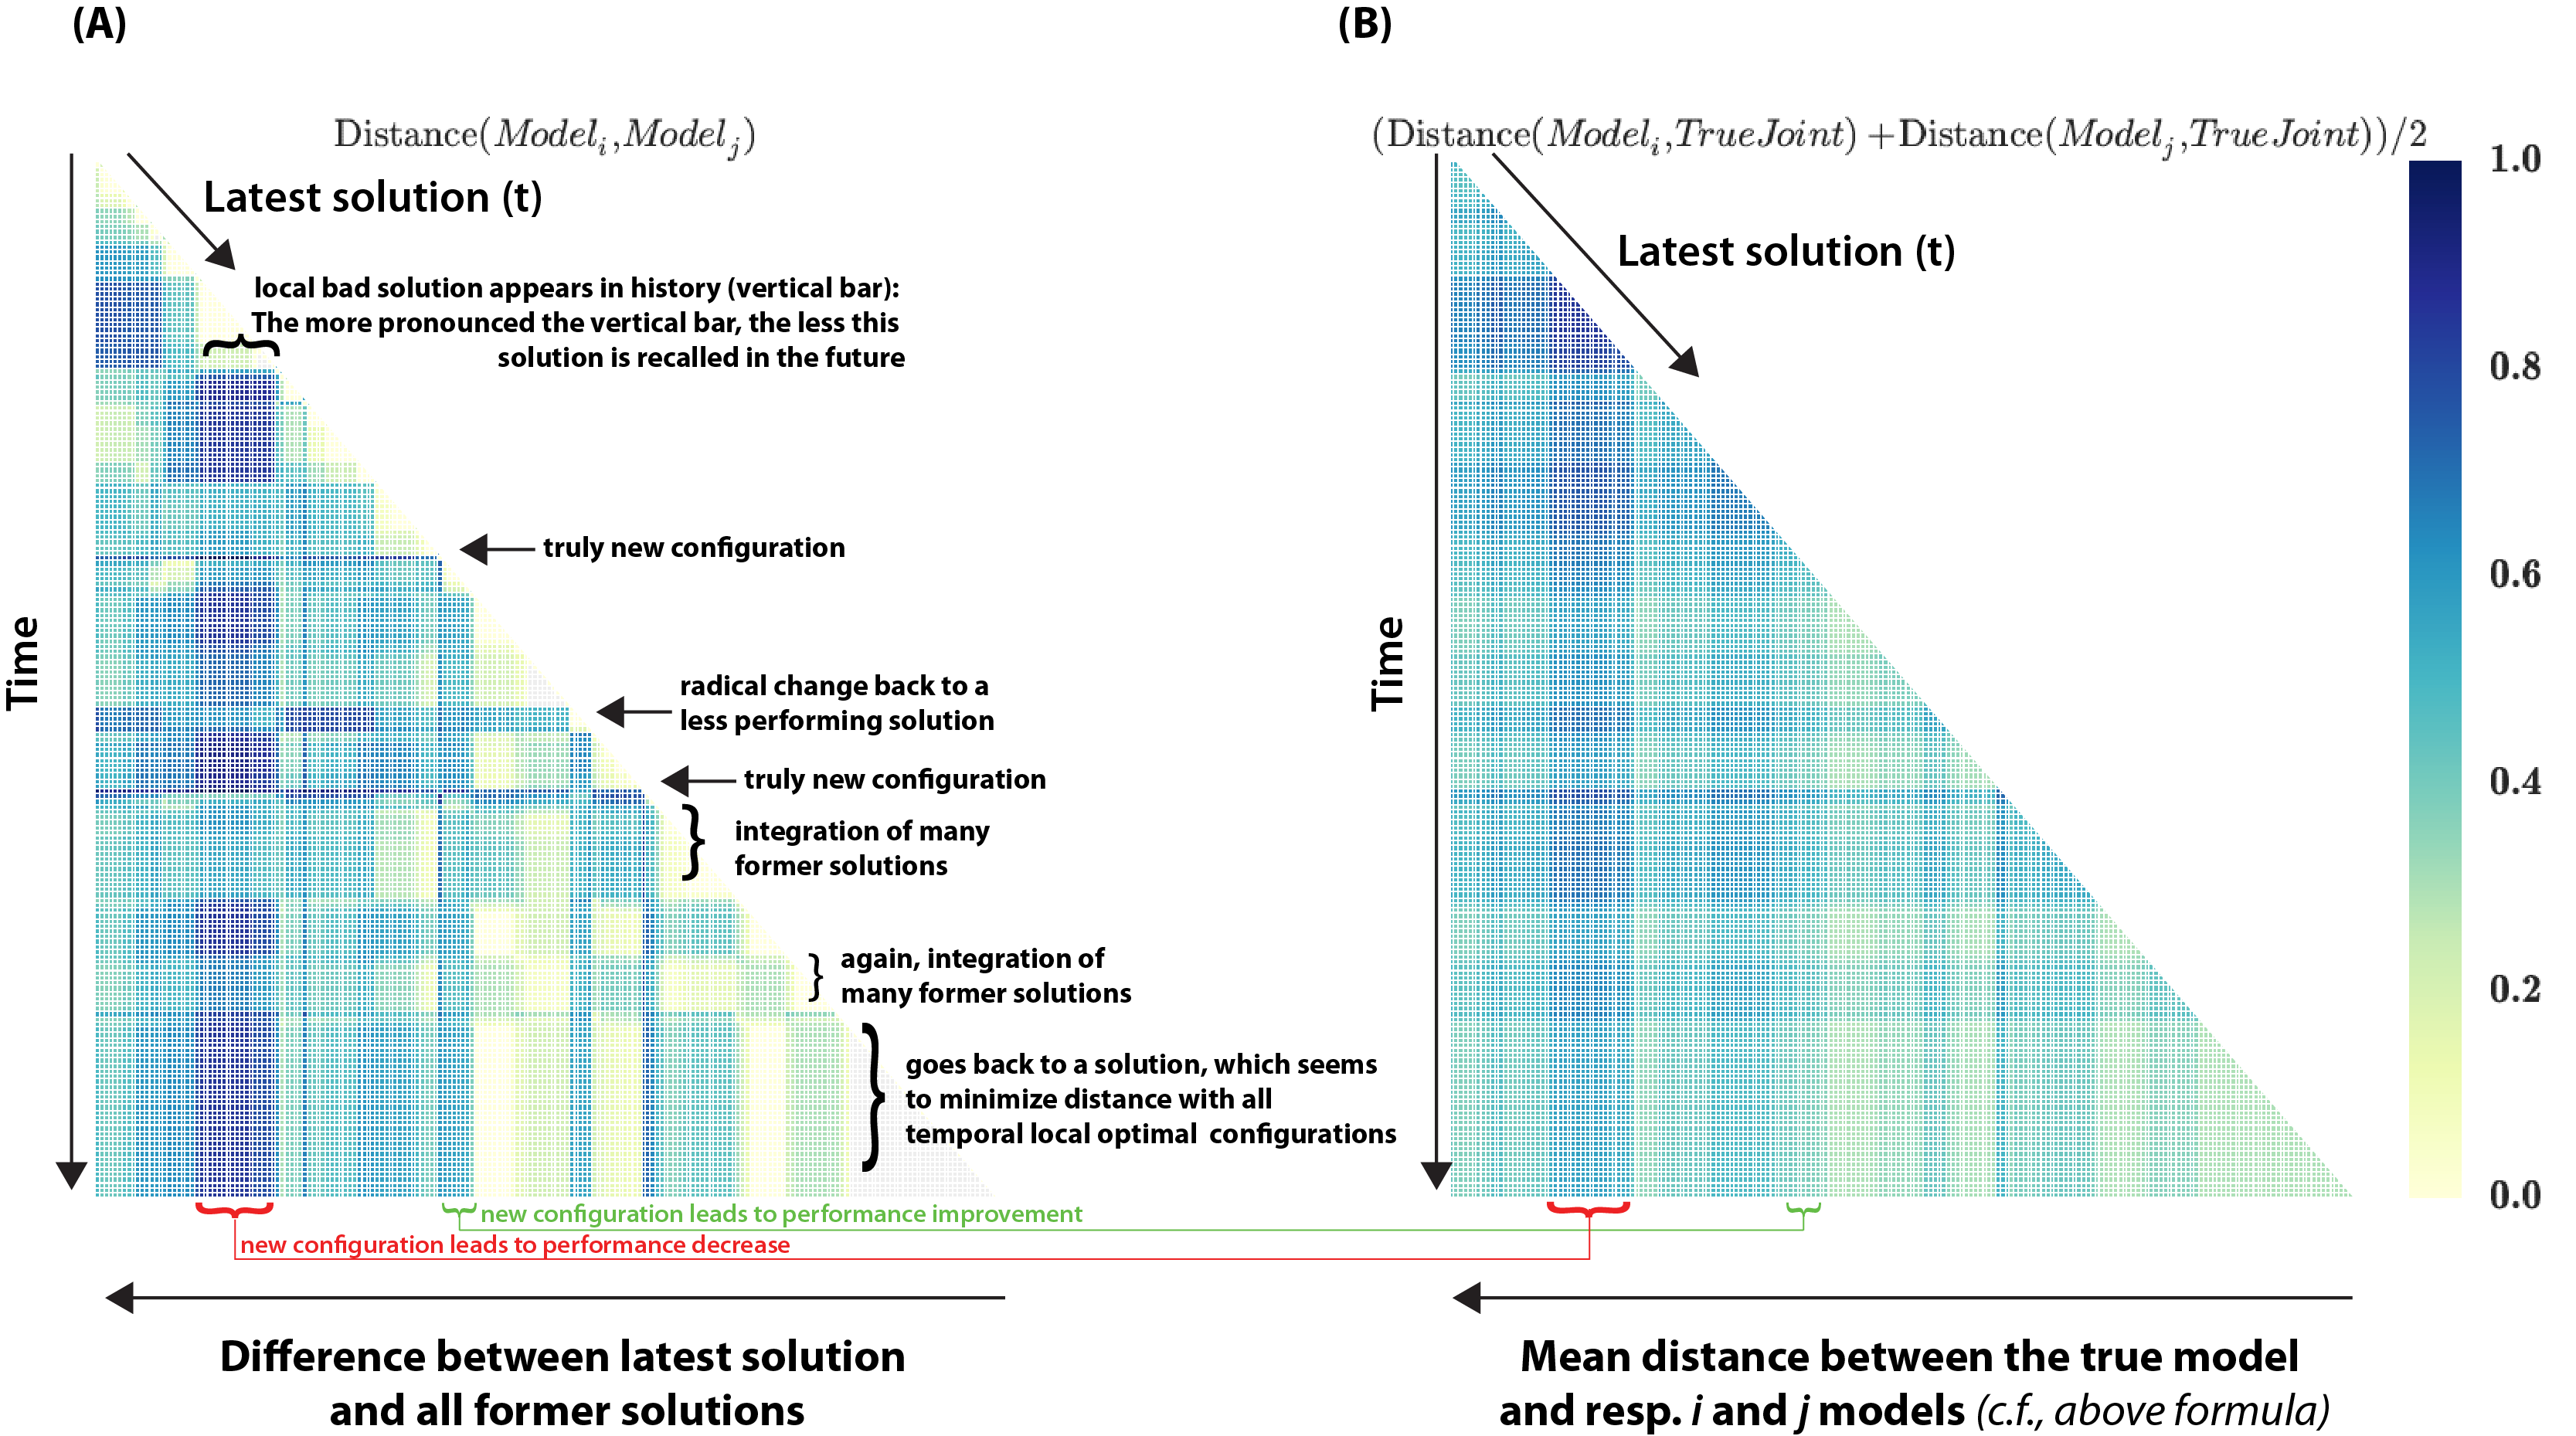
\includegraphics[width=0.98\columnwidth]{figures/matrice2/matrice2}
\caption{\label{fig:matrices}
Triangular matrices of difference between {\bf A} latest solution as a function of time and all former solutions, and {\bf B} of mean distance between the true model and resp. $i$ and $j$ configurations. Matrix {\bf B} shows the performance of a proposed model and serves as a reference for rationalizing choice sequences made by participants. These choice sequences are represented in matrix {\bf A} for participant 13: We see a wealth of characteristic choices leading to better of worse solutions, but also some integration and disruptive change in strategies, some which having a positive impact on performance, and other having a negative impact on performance. The rectangle structures show that participants do not drastically update drastically, but rather alternate periods of fine tuning and radical innovation. Matrix {\bf A} can also be watched in a more heuristic way at the coarse grained level: The more contrasted the pattern the more innovation overall. And, as shown here for participant 13, as more models are tested -- towards the lower right corner -- colors get more yellowish showing overall convergence of models. In the case presented here, the convergence of models leads overall to better solutions over time. It may not always be the case.%
}
\end{center}
\end{figure}

\section{Some ideas for a model}

It's a bit freestyle here, and we shall reconnect with theories in cognitive science, but the idea, is the following. 

There are two types of behaviors leading to their own dynamics
\begin{enumerate}
\item Optimization by small iterative steps
\item Disruptive innovations
\end{enumerate}
  
The former works almost as Bayesian learning, by the progressive integration of knowledge step by step (with some small try-and-fail), while the latter consists in jumping to new new places in the non-linear optimization space. However, the jump is not random, but builds on former experience either trying to {\it integrate} many former solutions found beforehand (yellowish horizontal stripes), or on the contrary, trying to find new solutions orthogonal to as many former solutions as possible (blueish horizontal strips). In both cases, we see that the outcome -- in terms of distance to the true model -- can be positive or negative.

\begin{table} 
    \begin{tabular}{ c c c }
         & positive outcome(improvement) & negative outcome(model worse than the best solution achieved so far) \\ 
        integrative model & X  & X \\ 
        orthogonal model & X &  X \\ 
    \end{tabular}
\label{tab:table}
\end{table}

From Figure \ref{fig:matrices}, it looks like for the game played in this experiment, radical changes have highest impact, and small changes seem to have negligible effects (it might be a result of the averaging formula employed). We shall therefore focus only on disruptive changes, their types (as described in Table \ref{tab:table}), their timing of these actions, and the resulting outcome.

Here are a few bullet points:
\begin{itemize}
\item Compute conditional probabilities of positive (resp.negative) outcome conditioned on {\it integrative} or {\it orthogonal} innovation. 
\item Look at timing of actions (not clear yet how to do this).
\end{itemize}







  
  
  

\section{Exploitation versus Exploration}



\subsection{Shall we consider the 8 dimensions together or indepedent?}

the distance measure is a well performing dimension reduction, I think.  It is hard to think in eight dimensions or to make visual graphs but by varying the weights for the past models for this measure one can explore more of this exploitation-exploration dynamic in dimensions related to more intuitive ideas, such as time.  Also, the eight dimensions are intricately correlated so that they can not be seen as independent dimensions and the measure of exploration-exploitation accounts neatly for the differences in beliefs about these correlation structures. 

\section{Next Steps}

\begin{enumerate}
\item {\bf Literature review}: Scott Page stuff (his work and the work he cites), Go more in depth in the James March (Management Science), Simon, H. The science of the artificials, Ch. 4. + Cognitive Science Guys
\item Get data for number 13 (simple), and then, for all individuals
\item Exploration (resp. Exploitation) phases (dis-improvement resp. improvement dynamics): (i) inspect phases qualitatively, (ii) chilling effect. Can we verify that indeed exploration (resp. exploitation) occurs during phases of disimprovement (resp. improvement). 
\item come up with a continuous metric between exploitation and exploration.
\item at the aggregate level it looks like these phases are more or less consistent across subjects: Is there a ``universal" (self-similarity) law governing exploration versus exploitation.
\item Is the process self-similar ?
\item peaks and valley $\rightarrow$ $\Delta Perf / \Delta t = (Peak - Valley)/(t_{Peak} - t_{Valley})$, with $Valley$ the last best performance and $Peak$ the next worst performance, then $\Delta Perf / \Delta t$ as a function of $T$.
\end{enumerate}


\section{Side ideas} 

\begin{enumerate}
\item modularity: you can think of brain packaging parameters and/or sub-optimal set of parameters of interest, which are recalled in congruent/coherent way.
\item 
\item
\end{enumerate}

\bibliography{bibliography/converted_to_latex.bib%
}

\end{document}

